\documentclass[twocolumn,12pt,a4paper]{article}

\usepackage[english]{babel}
\usepackage[utf8]{inputenc}
\usepackage[T1]{fontenc}
\usepackage{multicol}
\usepackage[top=3cm, bottom=3cm, left=2.5cm, right=2.5cm]{geometry}
\usepackage[bookmarks=true,bookmarksnumbered=true,hidelinks]{hyperref}
\usepackage{fancyhdr,lastpage}
\renewcommand{\footrulewidth}{0.4pt}
\usepackage[bf,sf]{titlesec}
\usepackage{siunitx}
\usepackage{titling,graphicx}
\usepackage{abstract}
\usepackage{amsmath}
\usepackage{siunitx}

\pagestyle{fancy}
\lhead{\textsf{Solar Sailing from Earth to Mars}}
\rhead{\textsf{Team 891}}
\cfoot{\thepage{} of \pageref*{LastPage}}

\setlength{\columnsep}{1.5cm}

% Numerar equacions amb la secció
\numberwithin{equation}{section}

\author{\textsf{Team 891}}
\title{\textsf{\textbf{Problem A: Solar Sailing from Earth to Mars}}}
\date{\textsf{November 12, 2017}}

\begin{document}
\renewcommand{\abstractname}{}
\renewcommand{\absnamepos}{empty}
\begin{titlingpage}
 \maketitle

\noindent \hrulefill \\
\begin{abstract}
Test test test

\end{abstract}
\hrulefill \\

\end{titlingpage}

\clearpage

\section{Introduction}

\subsection{Approach}
The motion of a solar sail within the Solar System, after a number of assumptions have been made, can be modeled by a set of relatively concise differential equations. Therefore, the problem at hand essentially becomes an initial value problem. 

As a first approximation, it can be found that a solar sail moves following as a logarithmic spiral. We used this fact to determine the feasibility of a trip from Earth to mars using solar sail propulsion, and to give a lower bound on the size of the sail for this trip to take a reasonable amount of time.

However, more complexity needed to be introduced to the model in order to understand the later stages of the trip, namely, from the point when the gravitational pull of Mars is no longer negligible. This means that the equations are no longer solvable analitically, so numerical methods must be used.

 A more detailed interpretation of the problem was needed so that a more precise model could be built. Understanding firstly the physical foundations around solar sailing was essential in order to perform an accurate analysis. Research has been done on the different forces affecting the sail for trajectories to be computed. Since some initial conditions are already given it has been necessary to verify whether these were the best options to accomplish the overall goal of the study or not.
 
  Moreover the aim of the survey is not only to calculate the path followed by the craft but also to determine its velocity so that a safe landing can be guaranteed. However, as trying to consider the attraction of Mars does not always give accurate results, this is not an easy task, though an estimate of craft arrival to Mars is presented at the end.
 
 It will be understood that the sail starts its trajectory with a radial velocity equal to the Earth's escape velocity, and with a tangential velocity equal to the Earth's linear velocity around the Sun. 
 
The release of the space craft will be considered at the time in which the Earth is closest to Mars, although, as it will be further discussed, results do not point in this being the best configuration. Since orbits of both planets are regarded as circular, as mentioned in the following section, this occurs when the Earth, Mars and the Sun are aligned.

The main goals of the article are to discuss a suitable distribuiton of the mass of the space craft, as well as to simulate possible trajectories and the arrival of the sail to Mars.

\subsection{Main assumptions}
To model the motion of a solar sail, we assumed it to be subject solely to the gravitational attraction from the Sun and solar radiation pressure. This yields a meaningful first approximation which can be used to gain insight on 

Throughout the article, several assumptions have been made, both as interpretations of the problem and in order to facilitate the model. However, all assumptions are supported by literature, and all the approximations were found to be reasonable. We present the approximations and interpretations made.

\begin{itemize}
\item The orbits of Mars and the Earth are coplanar and perfectly circular.
\item The only forces acting on the sail during its flight are the gravitational force exerted by the Sun and the thrust given by the inciding photons. Since the initial radial velocity is the Earth escape velocity, it is reasonable not to consider its attraction. In a first approach to the model, Mars attraction force has not been computed.
\item As stated in the problem given, we assume the total mass of the space craft is \SI{2 000}{kg} , including the payload and the sail. Thus, our goal is to maximize the payload while still finding a reasonable time of flight. 
\item Comparing the research which has already been done to the fact that the preassure exerted by light is twice its energy density, one finds that the case given is one of a perfect reflection.
\item We assume the only initial radial velocity of the sail is the Earth's linear velocity. Thus, one ignores the effects of the Earth's rotation.
\end{itemize}


\section{The physics of solar sailing}
We will follow \cite{tsu} and \cite{mcinnes} for most of this section.
\subsection{Radiation pressure}
It is well-known that electromagnetic wave carries an energy density. The fundamental idea behind solar sails is to use this energy as a means of propulsion in a way very much similar to how traditional sails take advantage of the kinetic energy of the wind. Given that the diameter of any reasonable solar sail will be much smaller than its distance to the Sun, one may approximate the solar radiation that arrives at the sail in the form of sinusoidal planar waves of frequency \( \omega \).

If \( E(t) \) is the amplitude of such waves, then the energy density, \( u \), they carry is given by \( u = \epsilon_0 E(t)^2 = \epsilon_0 E_0^2 \cos^2{\omega t} \). If one averages this over a period \( T \), then one obtains that the average energy density is simply \( \epsilon_0 E_0^2 /2 \), which can be rewritten as \( I/c \), where \( I \) is the intensity of the wave and \( c \) is the speed of light. Thus one finds that the pressure that incoming radiation exerts on the sail is \( I/c \). However, given that the material of the sail is not a black body, a fraction, \( R \), of the absorbed radiation will be emitted, giving rise to an additional term of pressure of the form \( RI/c \). If the sail is made out of a perfectly reflective material then it is the case that \( R = 1 \) and then the total pressure exerted on the sail is \( p = 2I/c \). This is the case for the problem at hand.

The intensity of a spherical wave is inversely proportional to the square of the distance from the source. Thus, the force exerted on the sail by the radiation from the Sun follows an inverse square law. We can make this dependence explicit by considering the equality \( Ir^2 = I_0 r^2_0 \), where \( I_0 \) is the intensity of solar radiation at a distance equal to the radius of the orbit of the Earth, \( r_0 \). And so we find that the force due to radiation pressure on a sail of surface area \( S \) is
\begin{equation}
 	\mathbf{F}_R(r) = \dfrac{2SI_0r_0^2}{c}\dfrac{1}{r^2} \mathbf{\hat{e}}_r \label{eq:radiation force}
\end{equation}

\subsection{Equations of motion for a solar sail: orthogonal case}
We have established that a solar sail that receives radiation in a direction orthogonal to itself experiences an inverse square central force. The other force acting on the sail is gravitational attraction due to the Sun ---we will consider the gravitational pull from other planets to be negligible when compared to that of the Sun---, which is also an inverse square force law. Namely:
\begin{equation}
 	\mathbf{F}_G(r) = -\dfrac{G M_S m}{r^2} \mathbf{\hat{e}}_r \label{eq:gravitational force}
\end{equation}
where \( m \) is the mass of the solar sail ---including the mass of the payload--- and \( M_S \) is the mass of the Sun.

Thus, we are now in a position to write the equations of motion for the solar sail
\begin{align}
	a_{r} &= \dot{v}_r - \dfrac{v_{\theta}^2}{r} = \dfrac{F_R - F_G}{m} \label{eq:equations of motion perpendicular} \\
	a_{\theta} &= \dot{v}_{\theta} + \dfrac{v_r v_{\theta}}{r} = 0 
\end{align}
It is common to introduce a number of parameters to better encapsulate the nature of a solar sail. The characteristic acceleration of a solar sail, \( a_R \), is defined to be the acceleration the sail experiences due to radiation pressure at a distance equal to 1 astronomical unit (AU) from the Sun. In keeping with the notation introduced in the previous section we write
\begin{equation} \label{eq:characterisit acceleration}
  a_R = \dfrac{2SI_0}{mc}
\end{equation}
It is then immediate to see that, if we denote the acceleration due to radiation pressure by \( a_R \) we have
\begin{equation}
  a(r) = a_R \dfrac{r_0^2}{r^2} 
\end{equation}
We can do the same with the acceleration due to gravity and we find
\begin{equation}
  a(r) = a_G \dfrac{r_0^2}{r^2} = \dfrac{G M_s}{r_0^2} \dfrac{r_0^2}{r^2}
\end{equation}
With this in mind we can then rewrite \autoref{eq:equations of motion perpendicular} as follows
\begin{align} \label{eq:equations of motion characteristic accelerations}
  \dot{v}_r - \dfrac{v_{\theta}^2}{r} &= (a_R - a_G) \left(\dfrac{r_0}{r}\right)^2 \\
	\dot{v}_{\theta} + \dfrac{v_r v_{\theta}}{r} &= 0
\end{align}
As we have already mentioned, this shows that the motion of a solar sail receiving radiation orthogonal to itself is governed by an inverse square law. In particular, the sail will move as if it were orbiting a star with a mass less than the Sun.

\subsection{Equations of motion for a solar sail: general case}
This, however, is only true if the sail is orthogonal to the incoming radiation. Indeed, if we allow for the sail to be at an arbitrary orientation, then its tangential acceleration is no longer zero. For this, we introduce the angle \( \alpha \), which is the angle between the vector normal to the sail, \( \hat{\mathbf{n}} \), and the radial direction. Now, the force due to radiation pressure has two contributions. The incoming photons exert a force that is now proportional to the orthogonal projection of the sail onto the radial direction, therefore of \( IS\cos{\alpha}/c \). This force is in the radial direction. The emitted photons exert a force that has the same modulus, but given that the sail behaves like a mirror, they are emmited in the direction orthogonal to the radial direction, and so the force due to the outgoing radiation is proportional to \( {-\hat{\mathbf{e}}_{\theta}} \). So we have
\begin{equation}
  \mathbf{F}_R(r) = \dfrac{2IS \cos{\alpha}}{c} ( \hat{\mathbf{e}}_{r} - \hat{\mathbf{e}}_{\theta})
\end{equation}
We now observe that because of symmetry, the vector \( \hat{\mathbf{e}}_{r} - \hat{\mathbf{e}}_{\theta}  \) is proportional to \( \hat{\mathbf{n}} \), and, because \( \hat{\mathbf{n}} \) is a unit vector then we have \( \hat{\mathbf{e}}_{r} - \hat{\mathbf{e}}_{\theta} = \cos{\alpha} \hat{\mathbf{n}} \). 
And thus we obtain
\begin{align}
  \mathbf{F}_R(r) &= \dfrac{2IS \cos^2{\alpha}}{c} \hat{\mathbf{n}} \\
									&= \dfrac{2IS \cos^2{\alpha}}{c} (\cos{\alpha} \hat{\mathbf{e}}_r + \sin{\alpha} \hat{\mathbf{e}}_{\theta}) 
\end{align}

Finally, we can rewrite the equations of motion for a solar sail in this more general case as follows:
\begin{align} \label{eq:equations of motion general case}
  \dot{v}_r - \dfrac{v_{\theta}^2}{r} &= (a_R \cos^3{\alpha} - a_G) \left(\dfrac{r_0}{r}\right)^2 \\ 
  \dot{v}_{\theta} + \dfrac{v_r v_{\theta}}{r} &= -a_R	\sin{\alpha} \cos^2{\alpha} \left(\dfrac{r_0}{r}\right)^2
\end{align}
As a consistency check,  we note that if \( \alpha = 0 \), that is, the sail is orthogonal to the radiation, we recover \autoref{eq:equations of motion characteristic accelerations}. However, the equations we have just obtained are \emph{not} the equations for a particle experiencing central force motion.   

\section{First Results}
\subsection{Feasibility of the trip}
To solve \autoref{eq:equations of motion general case} it is common to assume \( \dot{v}_r = 0\), as done in \cite{tsu} and \cite{mcinnes}. Then, the equations become those of a logarithmic spiral. Then, \( v_r = \dot{r} \) can be isolated and then integrated to find an expresssion for the time of travel between two orbits of a given radius in terms of only the parameters \( \alpha \), \( a_R \) and \( a_G \):

\begin{equation} \label{eq:time of flight between orbits}
	t=\frac{1}{3}\cdot\frac{r_0^{3/2}-r^{3/2}}{r_0\sqrt{a_R}}\cdot\frac{(a_G/a_R-\cos^3\alpha)^{1/2}}{\sin\alpha\cos^2\alpha}
\end{equation}

According to what has been discussed in the previous section, there are some variables of the sail which have to be calculated. This are
\[
a_R=6,45\cdot 10^{-7} \cdot m_s
\]
\[a_G=5,928\cdot 10^{-3}
\]
where $m_s$ denotes the mass of the sail.
Another parameter
Literature suggests \cite{tsu} one can neglect the  $\dot{v}_r$ term in equation \ref{carlessexy} as a first approach. The simplified equation reads
\begin{equation}
- \dfrac{v_{\theta}^2}{r} = (a_R \cos^3{\alpha} - a_G) \left(\dfrac{r_0}{r}\right)^2
\end{equation} 
which can be directly solved.

Having solved both velocities, one finds the trajectory taken is a logarithmic spiral, which only depends on the ratio \(a_G/a_R\) and $\alpha$.
Figure 1 shows a first approximation of the trajectory taken by the space craft with the mentioned suppositions and values.

\begin{figure}[h]
	\centering
	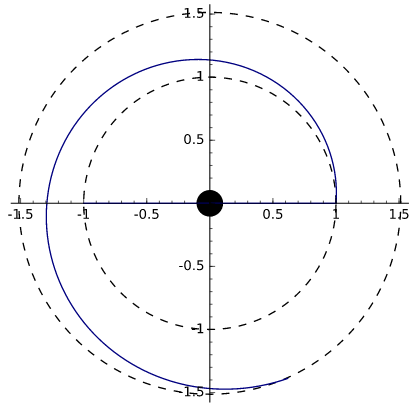
\includegraphics[scale=0.5]{espiral.png}
	\label{espiral}
	\caption{\small First approximation of the sail trajectory, in blue. The Sun is in the middle and the dashed lines represent the orbits of the Earth and Mars. Axis in AU.}
	
\end{figure}


Solving Equation 3.1 for $v_{\theta}$ and directly integrating, one can find the time of travel between radii $r_0$ and $r$.
In order to optimize the flight time it is useful to define the solar sail lightness number which can be calculated as
\begin{equation}
	\beta=\frac{a_R}{a_G}
\end{equation}
Using the last two expressions one can find that minimising timeflight implies minimising function of $\alpha$
\begin{equation}
	\frac{(1-\beta\cos^3\alpha)^{1/2}}{\beta\cos^2\alpha\sin\alpha}
\end{equation}
Imposing the condition that its derivative must be equal to zero one obtains
\begin{equation}
	\beta-\frac{2}{\cos\alpha}\frac{1-2\tan^2\alpha}{2-\tan^2\alpha}=0
\end{equation}
\begin{figure}[h] \label{fig:arnauoficinista}
	
	\centering
	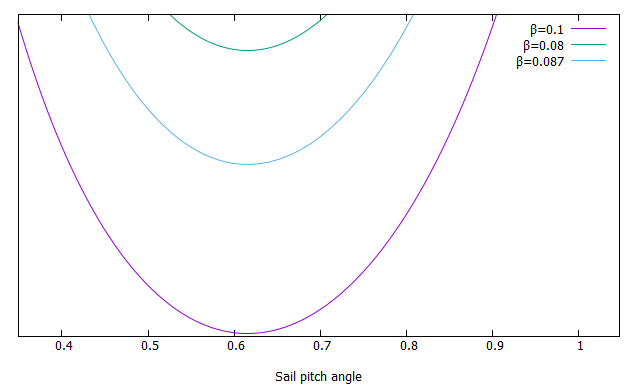
\includegraphics[scale=0.3]{angle.png}
	\caption{\small Different values for the function of $\alpha$}
\end{figure}
Computing for the optimal sail pitch angle one finds sligtly different values depending on $\beta$. Nevertheless, looking at \autoref{fig:arnauoficinista} one notices that for similar $\beta$ numbers the optimal angles are around $\alpha=0.62$ rad. Now, the only unknown variable in the time flight formula is the mass of the solar sail $m_s$.

Obviously, the time flight will decrease as the mass of the solar sail becomes bigger as this implies a bigger surface and as a consequence a bigger thrust. This fact is shown in \autoref{fig:time}.
\begin{figure}[h]
	\centering
	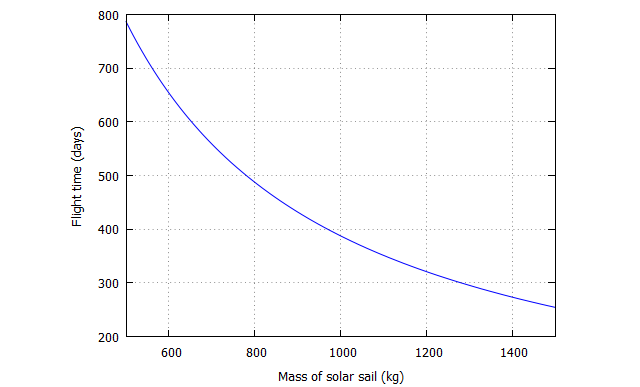
\includegraphics[scale=0.35]{time}
	\caption{\small Decrease of the flight time as a function of thet  solar sail mass}
	\label{fig:time}
\end{figure}

Firstly, it must be stated that with a maximum payload of $2000$kg one cannot safely send a manned space craft. Therefore, we will consider a mission consisting on sending just material.

One must now decide on a formula which will have both a reasonable time of travel and a sufficient amount of payload so that the mission is profitable. Researching past missions to Mars, time travels of about one year are reasonable and, to have an idea, a rover like Curiosity weights about $900$kg. Of course, extra material is needed, but, according to research, $1000$kg of payload seems a reasonable choice. From equation 3.2 it is found that the flight time will be around 390 days, which, as stated, seems feasible.

Choosing to distribute equally the mass of the sail and the mass of the sail, one gets a value for the solar sail lightness of $\beta=0.1088$. From now on, this value will be assumed to be equal to 0.1, since most of the other characteristics can be found in literature for such value.

However it is not enough to ensure a change of orbit, Mars position must be determined in order to desing an hypothetical landing. Some values regarding speed of the craft and its relative position to Mars are given to discuss this. Equations of motion can be solved according \cite{mcinnes} -page 155- where a explicit solution for $r(\theta)$ can be found. Having this, one finds that it takes around $4.7$ rad to perform the orbit change. Even so, this does not guarantee an encounter with Mars as by assuming its velocity to be constant its final position can be calculated. Considering the flight time, the angle between the radius vectors that define its initial and final position turns out to be $3.6$ rad. This is not an extremely accurate estimation as a perfect cirular orbit of Mars has been suposed.

 As a consequence, different options can be thought in order to solve this. The first one may consist in modifying the followed path by finding a secondary thrust source though attending to allowed payload this does not seem viable. On the other hand, a different initial condition could be considered in order to compensate the final angle difference between the craft and Mars. This will consist in launching the solar sail not at the closest approach to Mars but with an initial phase difference so that an encounter can be guaranteed. Nevertheless, this idea will not be developed in the survey as a better performance with this initial conditions is assessed in the following sections.
 
 Notwithstanding, thinking about using a different flight time suggests a better option. Taking the optimal sail pitch angle implies a fixed value of the flight time which in fact, is the minimal one. However, a greater time may be used in order to achieve a better approach to Mars.
\section{No sé quin títol}
\subsection{First simulation?}
Solutions of equations \ref{carlessexy} and \ref{carlessexy2} have been simulated. Figure ?? shows the trajectory followed by the sail. It is direct that it is still a spiral, but not a logaritmic one as in Figure \ref{espiral}. Note that the trajectory of the sail is not tangent anymore to the orbit of Mars.

The simulation also allows us to find a first approximation of the velocity with which the sail reaches Mars. Without considering the gravitational pull exerted by Mars, and approximating both curves to tangent, the relative velocity between both bodies is $-4km/s$, meaning Mars, which is behind the sail, reaches the spacecraft at a speed of $4$km/s.


\bibliographystyle{ieeetr}
\bibliography{UphysicscNotes}

\end{document}

